\subsection{Higgs physics at the LHC}
\label{higgs}

One important physics purpose of the LHC is searching for the Higgs boson, which was the last missing part in the SM.
This section will talk about both the production and decay modes of the SM Higgs boson in proton-proton collision.

%% ================================ Higgs production ===============================
\textbf{Higgs productions}

The Higgs boson can be produced through several processes.
There are 4 main production modes at the LHC: gluon-gluon Fusion (\textit{ggF}), vector boson Fusion (\textit{VBF}),
associated production with vector-bosons (\textit{VH}) (also called the Higgs Strahlung) 
and associated production with a pair of top/anti-top quarks (\textit{ttH})~\cite{Grojean:2243593}.
Figure~\ref{fig:higgs_productions_fd} shows the corresponding Feynman diagrams of each process (at LO).
\begin{figure}[!htb]
  \centering
  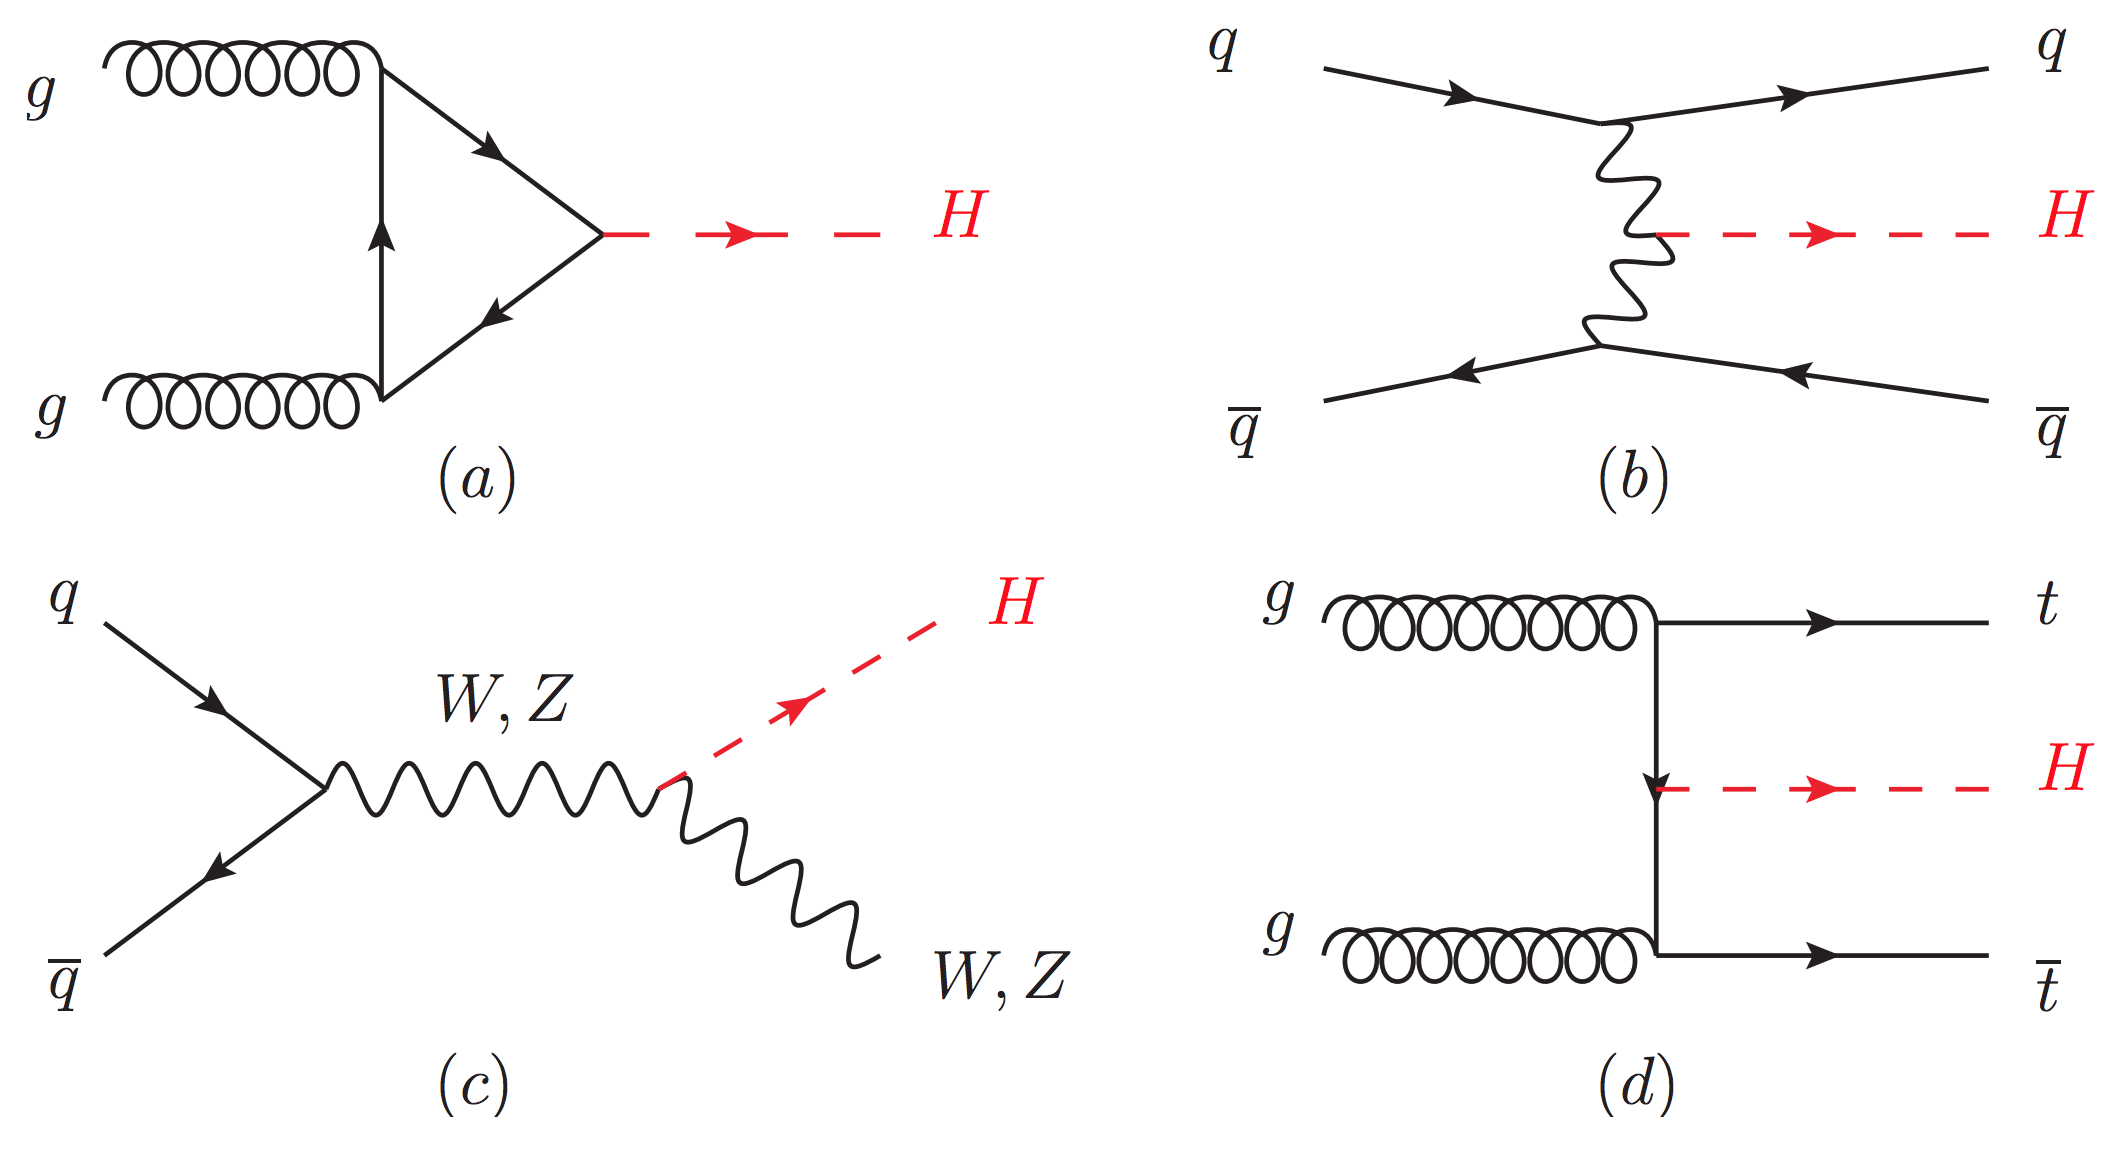
\includegraphics[width=0.8\textwidth]{figures/Theory/Figures_FeynmanHprod.png}
  \caption{Feynman diagrams of the Higgs production modes:
	   (a) ggF; (b) VBF; (c) VH; (d) ttH.}
  \label{fig:higgs_productions_fd}
\end{figure}
For pp collision, the cross section of productions of Higgs boson is as a function of centre-of-mass energy $\sqrt{s}$. 
Figure~\ref{fig:higgs_productions_xs} depicts the cross section of SM Higgs, whose mass is 125 GeV, for several different production modes when centre-of-mass energy varying from 6 to 15~\tev.
Figure~\ref{fig:higgs_productions_xs2} shows the prospect of production cross section  
as a function of Higgs mass from 10 to 2000~\gev~for pp collision at the centre-of-mass energy of 13~\tev~ and 14~\tev~ \cite{deFlorian:2227475}. 
\begin{figure}[!htb]
  \centering
  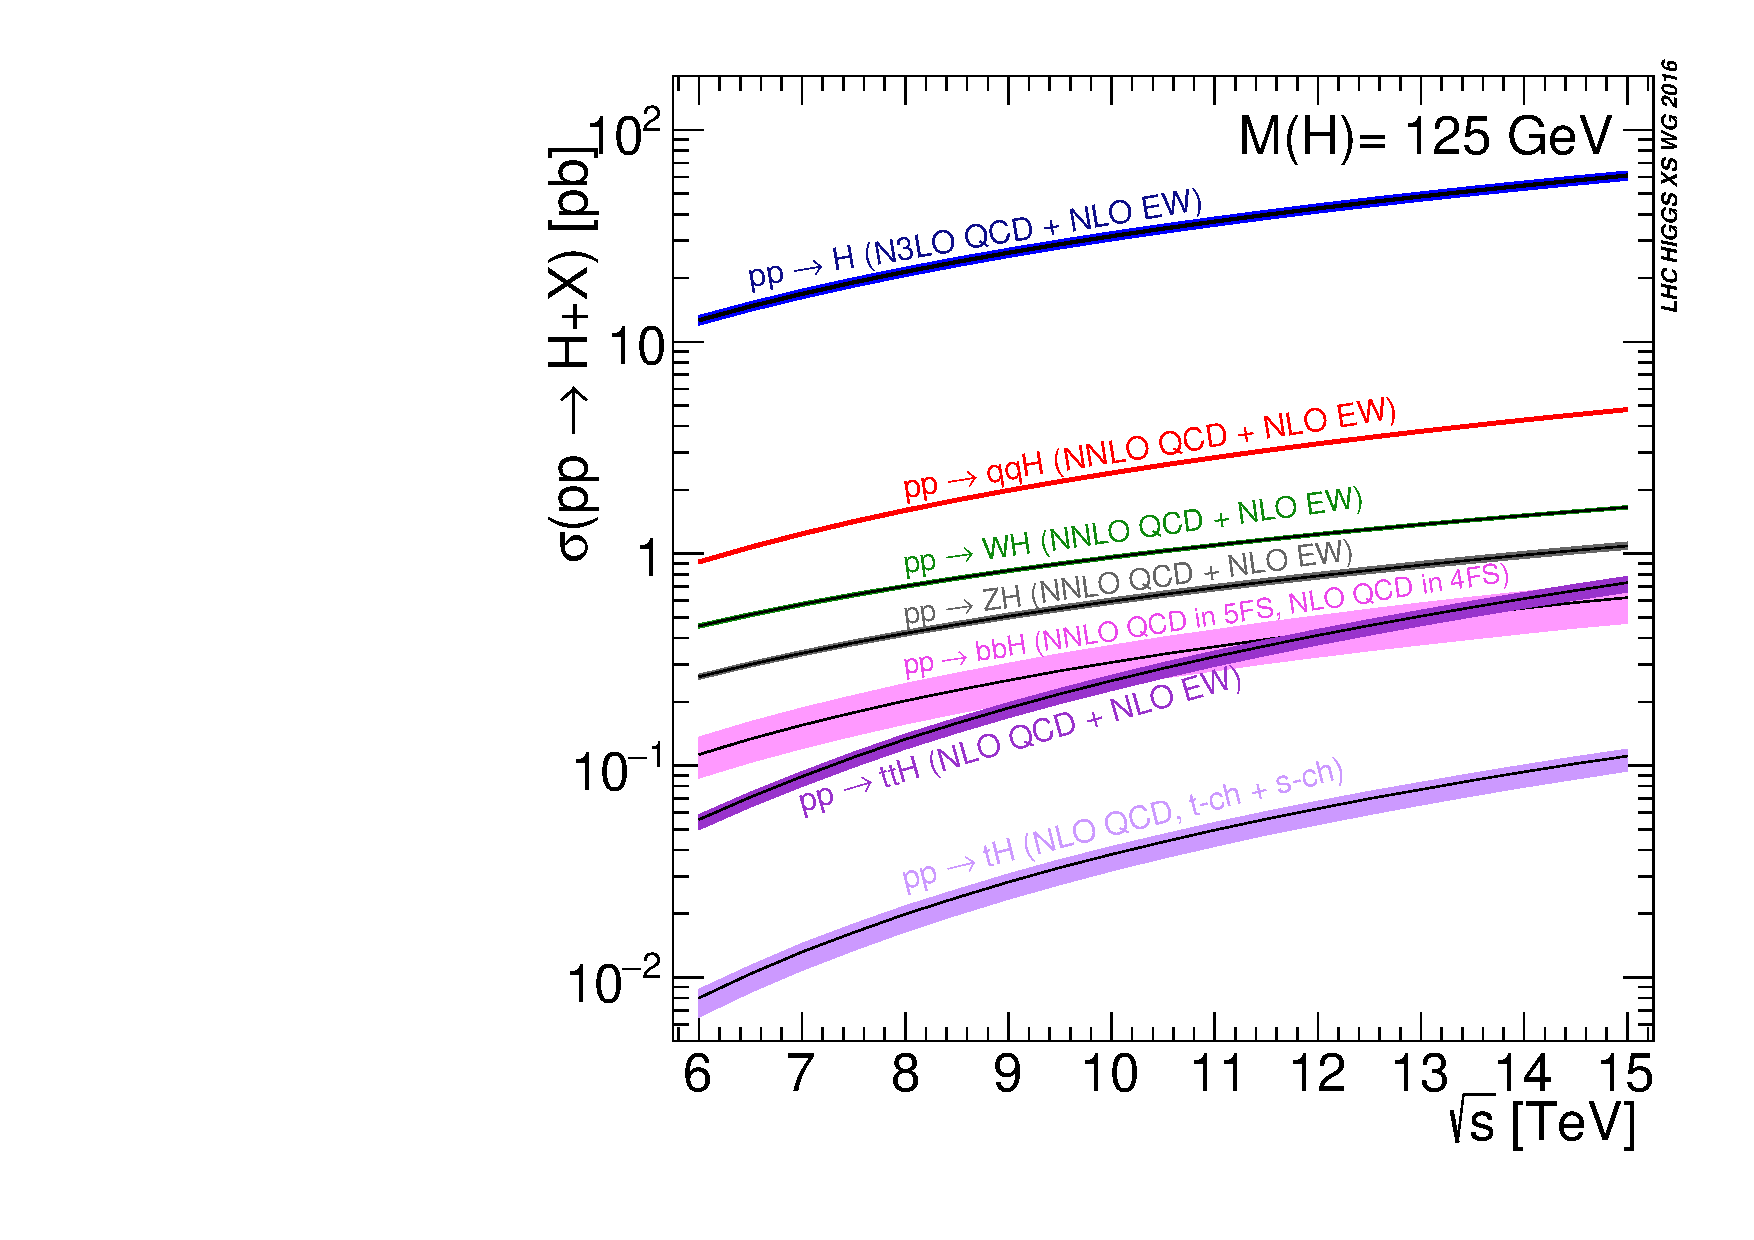
\includegraphics[width=0.5\textwidth]{figures/Theory/Plot_Escan_H125_new_sqrt.pdf}
  \caption{The SM Higgs boson production cross sections for various production modes as a function of the centre-of-mass energy for pp collision.}
  \label{fig:higgs_productions_xs}
\end{figure}
\begin{figure}[!htb]
  \centering
  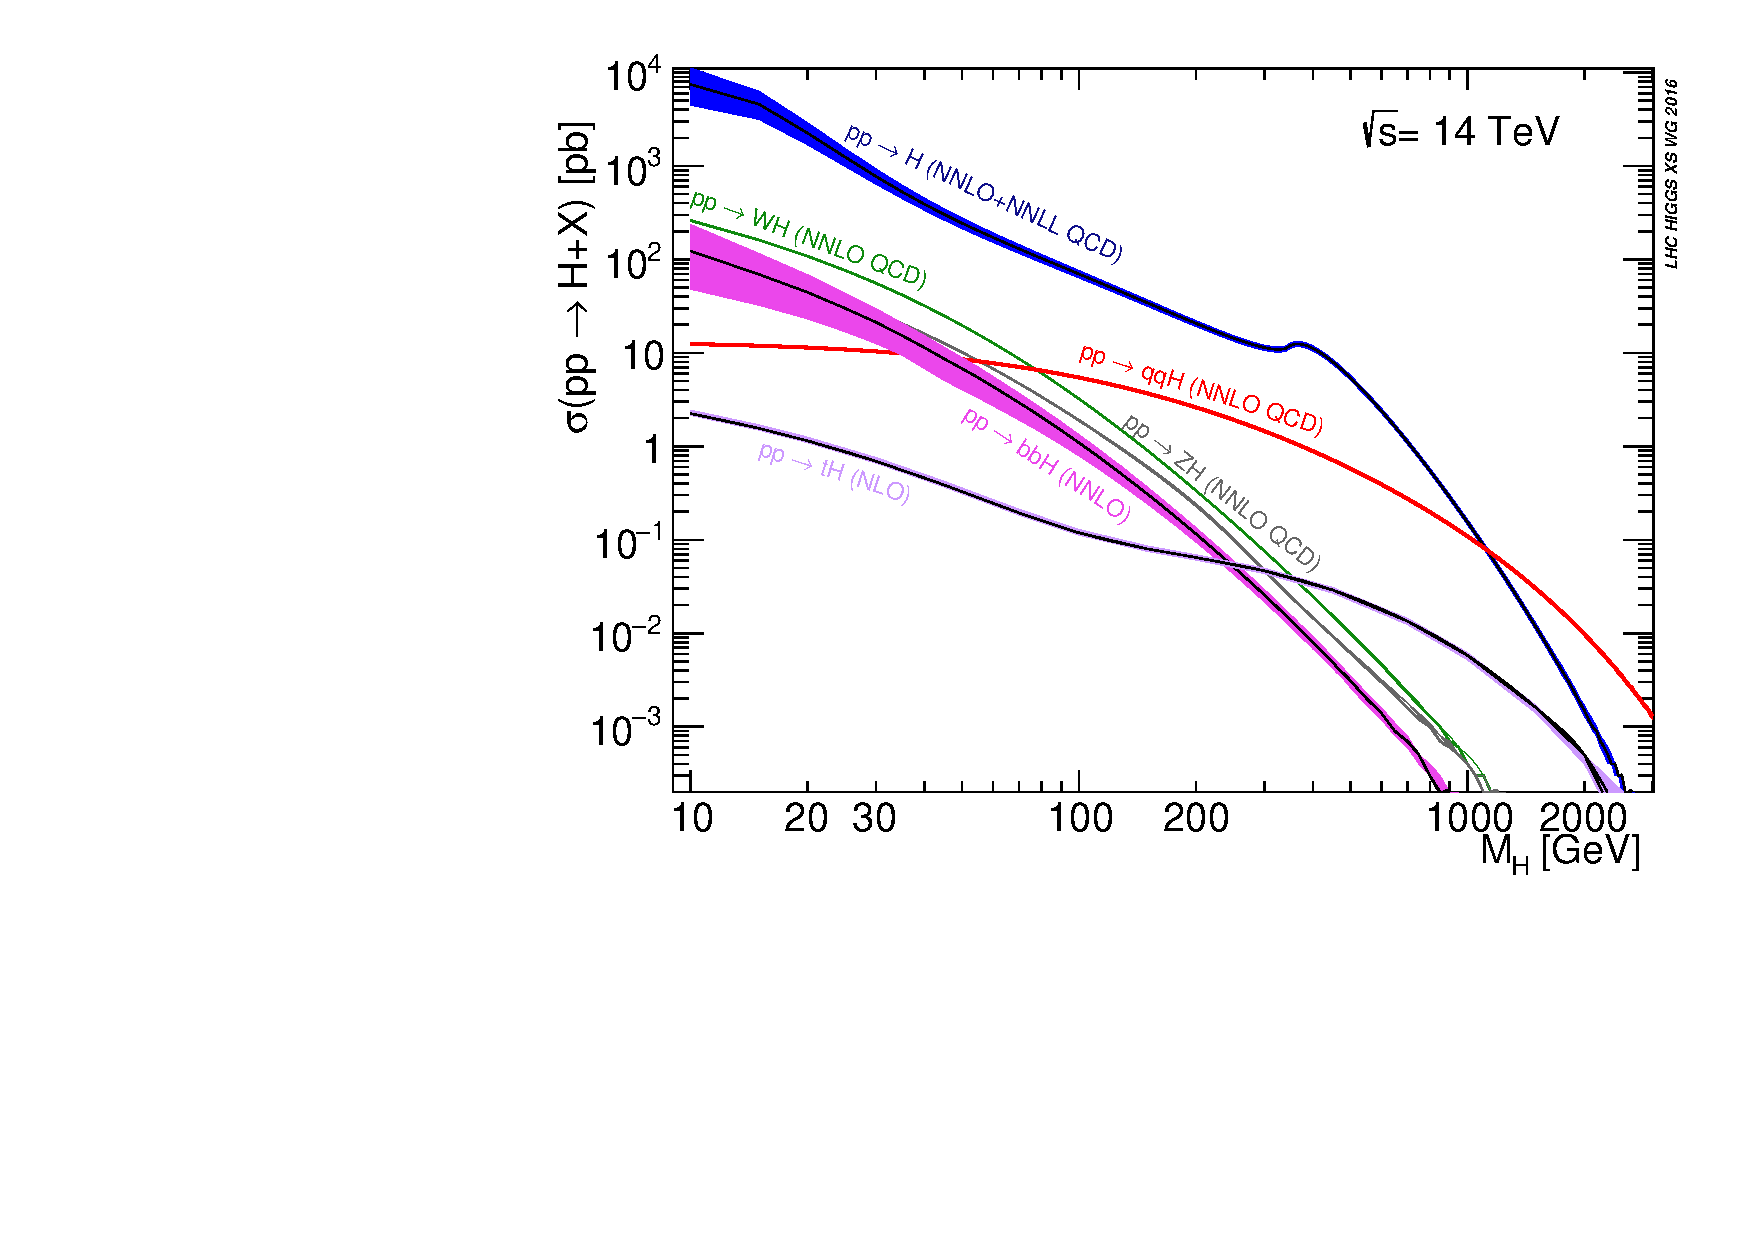
\includegraphics[width=0.45\textwidth]{figures/Theory/plotAll_14tev_BSM_sqrt.pdf}
  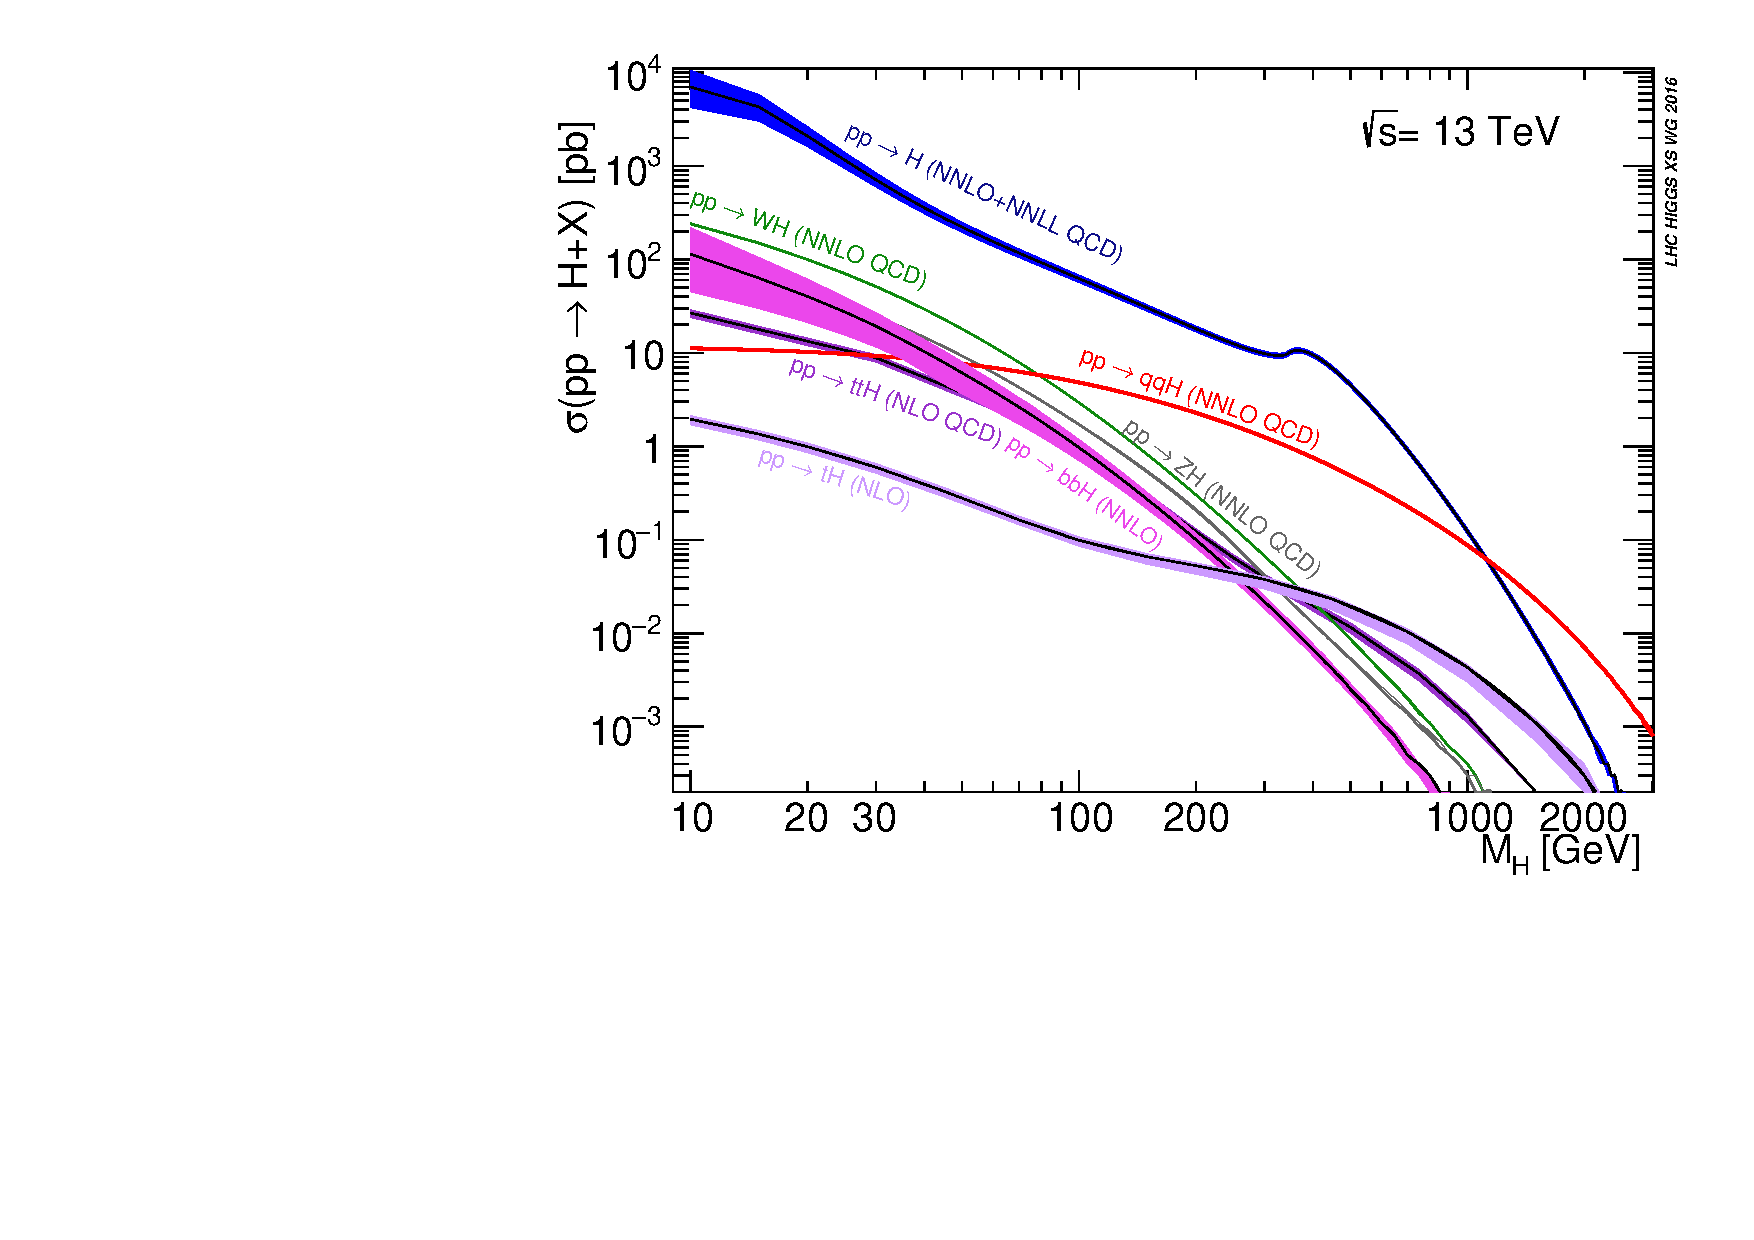
\includegraphics[width=0.45\textwidth]{figures/Theory/plotAll_13tev_BSM_sqrt.pdf}
  \caption{Higgs boson production cross section for various production modes as a function of the Higgs mass for $\sqrt{s}$ = 13~\tev~ (left) and 14~\tev~ (right) for pp collision.}
  \label{fig:higgs_productions_xs2}
\end{figure}

%% ================================ Higgs decays ===================================
\textbf{Higgs decays}

The Higgs boson can interact with gauge bosons and fermions through gauge coupling and the Yukawa coupling as introduced in section~\ref{symbreaking}.
Figure~\ref{fig:higgs_decay_fd} depicts the Feynman diagrams of various possible Higgs decay channels.
\begin{figure}[!htb]
  \centering
  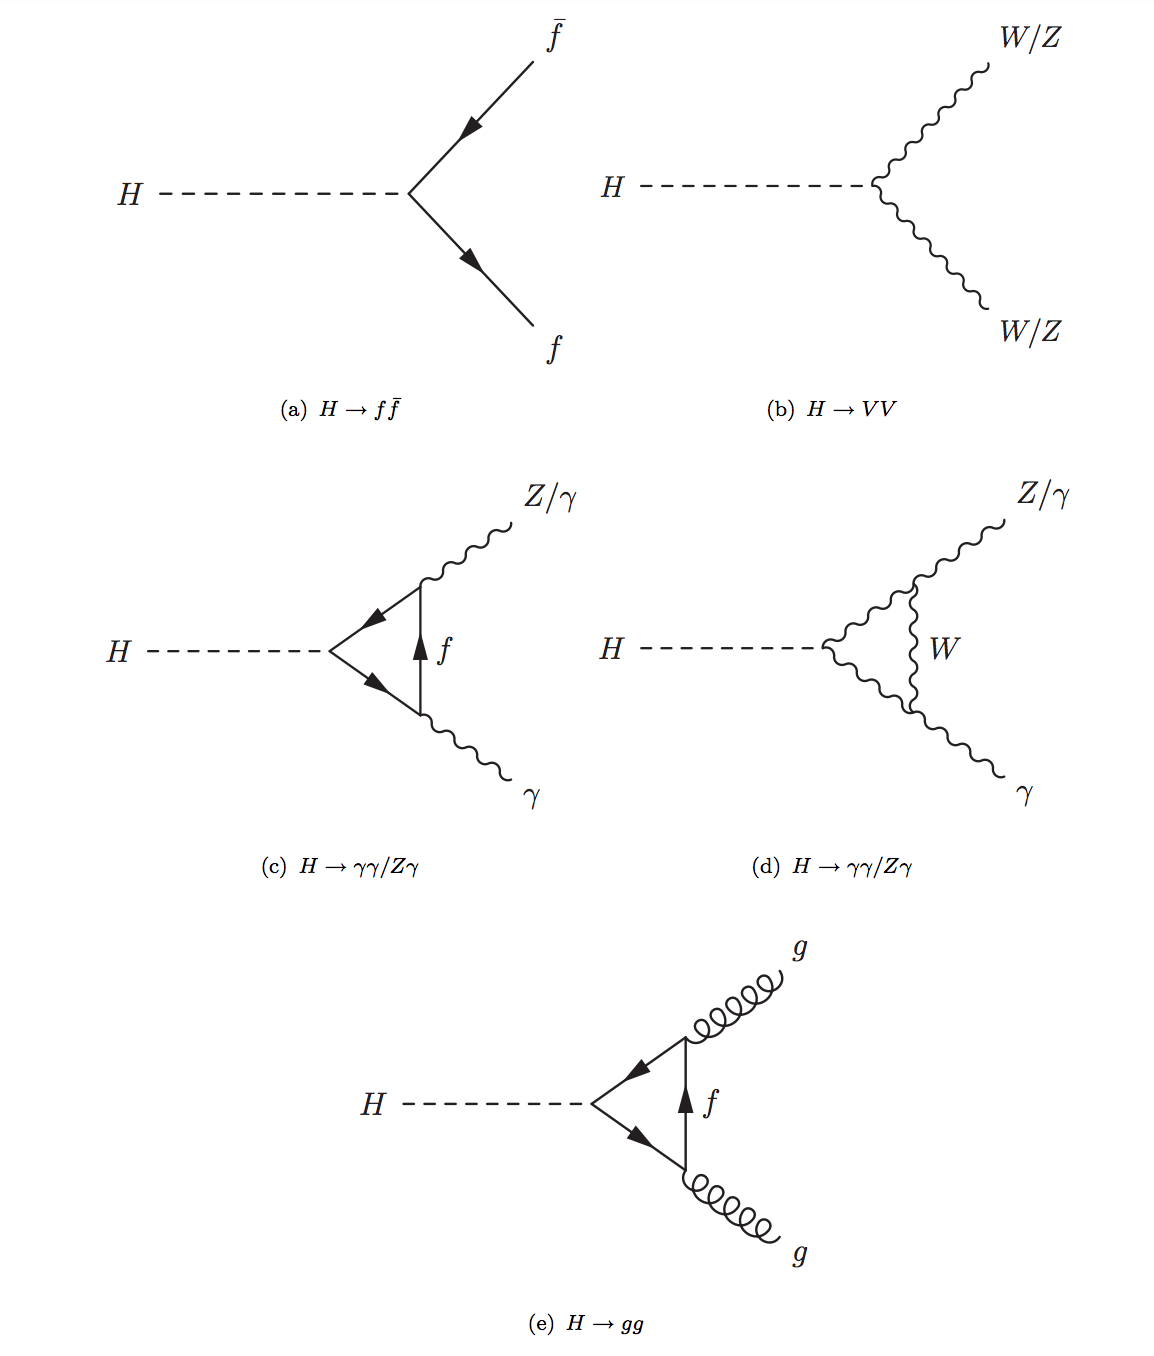
\includegraphics[width=0.8\textwidth]{figures/Theory/Figures_Feynman_Hdecay.png}
  \caption{SM Higgs decay channels.}
  \label{fig:higgs_decay_fd}
\end{figure}
The branching ratio of Higgs boson decaying into different final states as a function of Higgs mass is shown in figure~\ref{fig:higgs_decay_br}.
\begin{figure}[!htb]
  \centering
  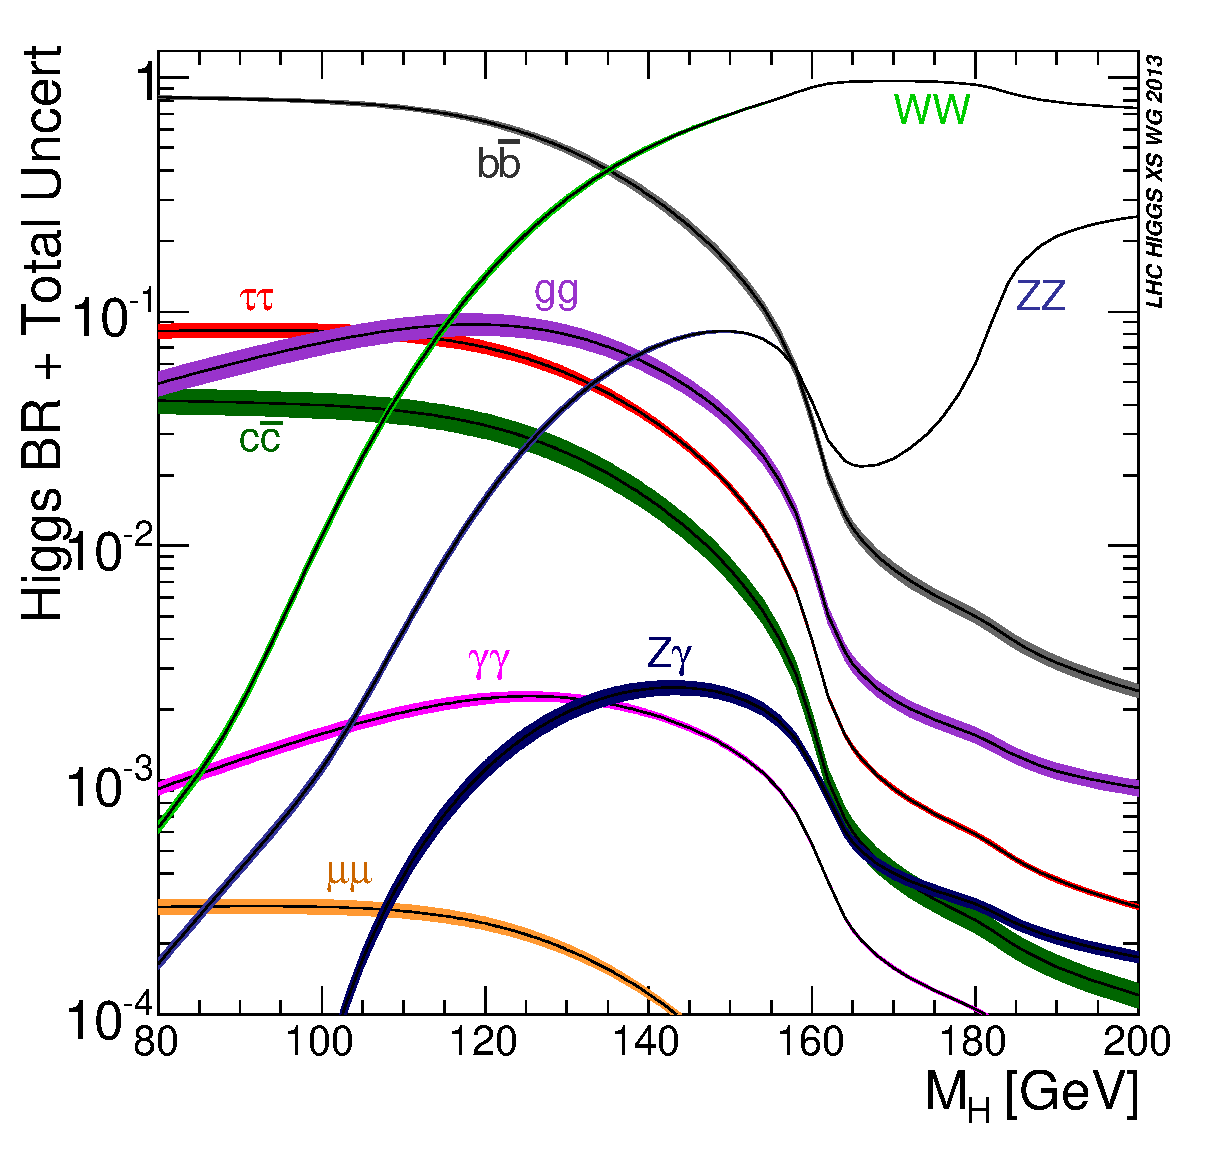
\includegraphics[width=0.5\textwidth]{figures/Theory/Higgs_BR_LM.eps}
  \caption{Branching ratio of Higgs decays in various channels as a function of Higgs mass~\cite{Heinemeyer:1559921}. }
  \label{fig:higgs_decay_br}
\end{figure} 

%% ====================================== High mass related ===========================
%(\textbf{BSM Higgs models})


